\lecture{7}{23 Sep. 15:30}{}
\begin{definition}[Ferrers diagram]
    Visual representation of \(\lambda \vdash n\). Each \(\lambda _i\) pirctured as a row of \(\lambda _i\) dots.    
\end{definition}
\begin{figure}[H]
    \centering
    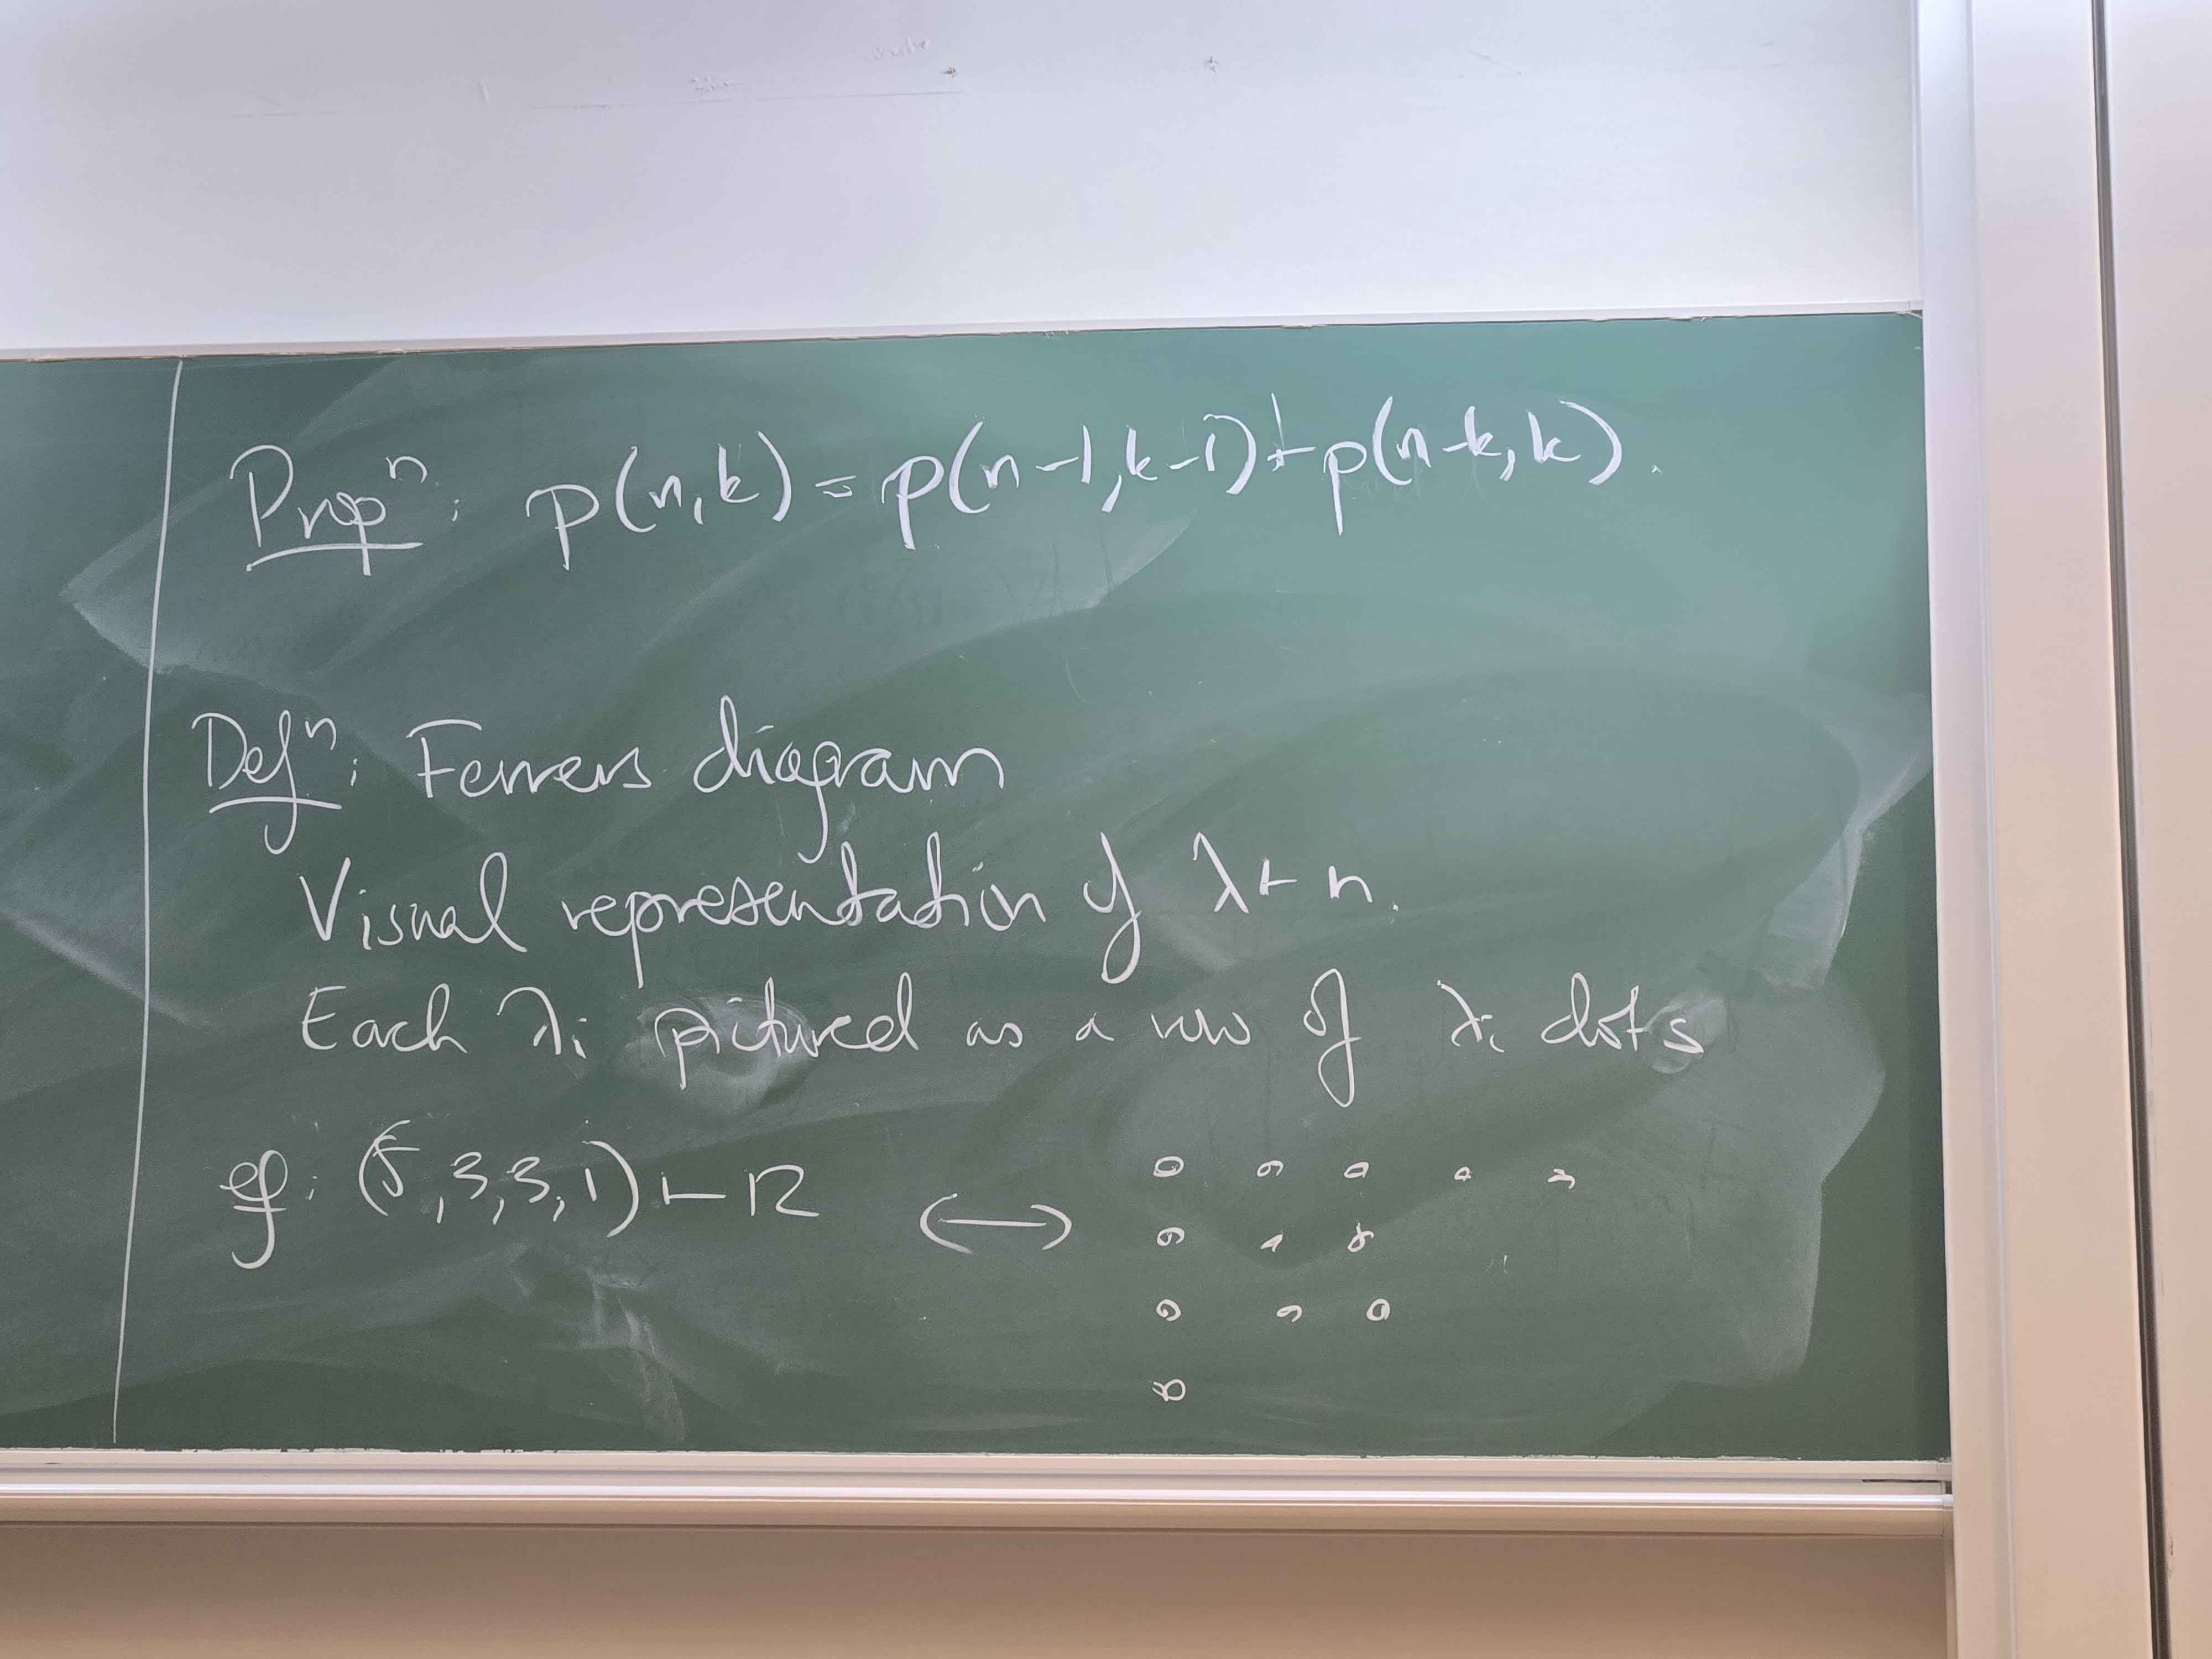
\includegraphics[width=0.7\textwidth]{./Figures/20250923_153141.jpg}
    \caption{Ferrers diagram}
    \label{fig:Ferrers}
\end{figure}

\begin{note}
    If we see the Ferrers diagram from the columns, then note that the number of dots in the columns is decreasing.
\end{note}

\begin{definition}
    Given a parition \(\lambda \vdash n\), the conjugate partition \(\lambda ^* \vdash n\) is given by 
    \[
        \lambda _j^* = \left\vert \left\{ i: \lambda _i \ge j \right\}  \right\vert. 
    \] 
    Visually, \(\lambda ^*\) is the partition obtained by reflecting \(\lambda  \) in the diagonal \(y = -x\).     
\end{definition}

Observe that \(\lambda ^*\) is indeed a partition of \(n\):
\[
    \lambda _1^* \ge \lambda _2^* \ge \dots 
\] is obvious from the definition, and 
\[
    \sum_{j} \lambda_j ^* = \sum_{j} \left\vert \left\{ i: \lambda _i \ge j \right\} = \sum_{i} \lambda _i = n   \right\vert.   
\]
Also, note that \(\left( \lambda ^* \right)^* = \lambda \). 

\begin{proposition}
    The number of partition of \(n\) into at most \(k\) parts \(=\) The number of partitions of \(n\) into parts of size \(\le k\).     
\end{proposition}
\begin{proof}
    The largest part of \(\lambda \) is the number of parts in \(\lambda ^*\). And so conjugation gives a bijection between these two choices of partition of \(n\).   
\end{proof}

\begin{definition}
    A parition \(\lambda \vdash n\) is called self-conjugate if \(\lambda  ^* = \lambda \).  
\end{definition}
\begin{figure}[H]
    \centering
    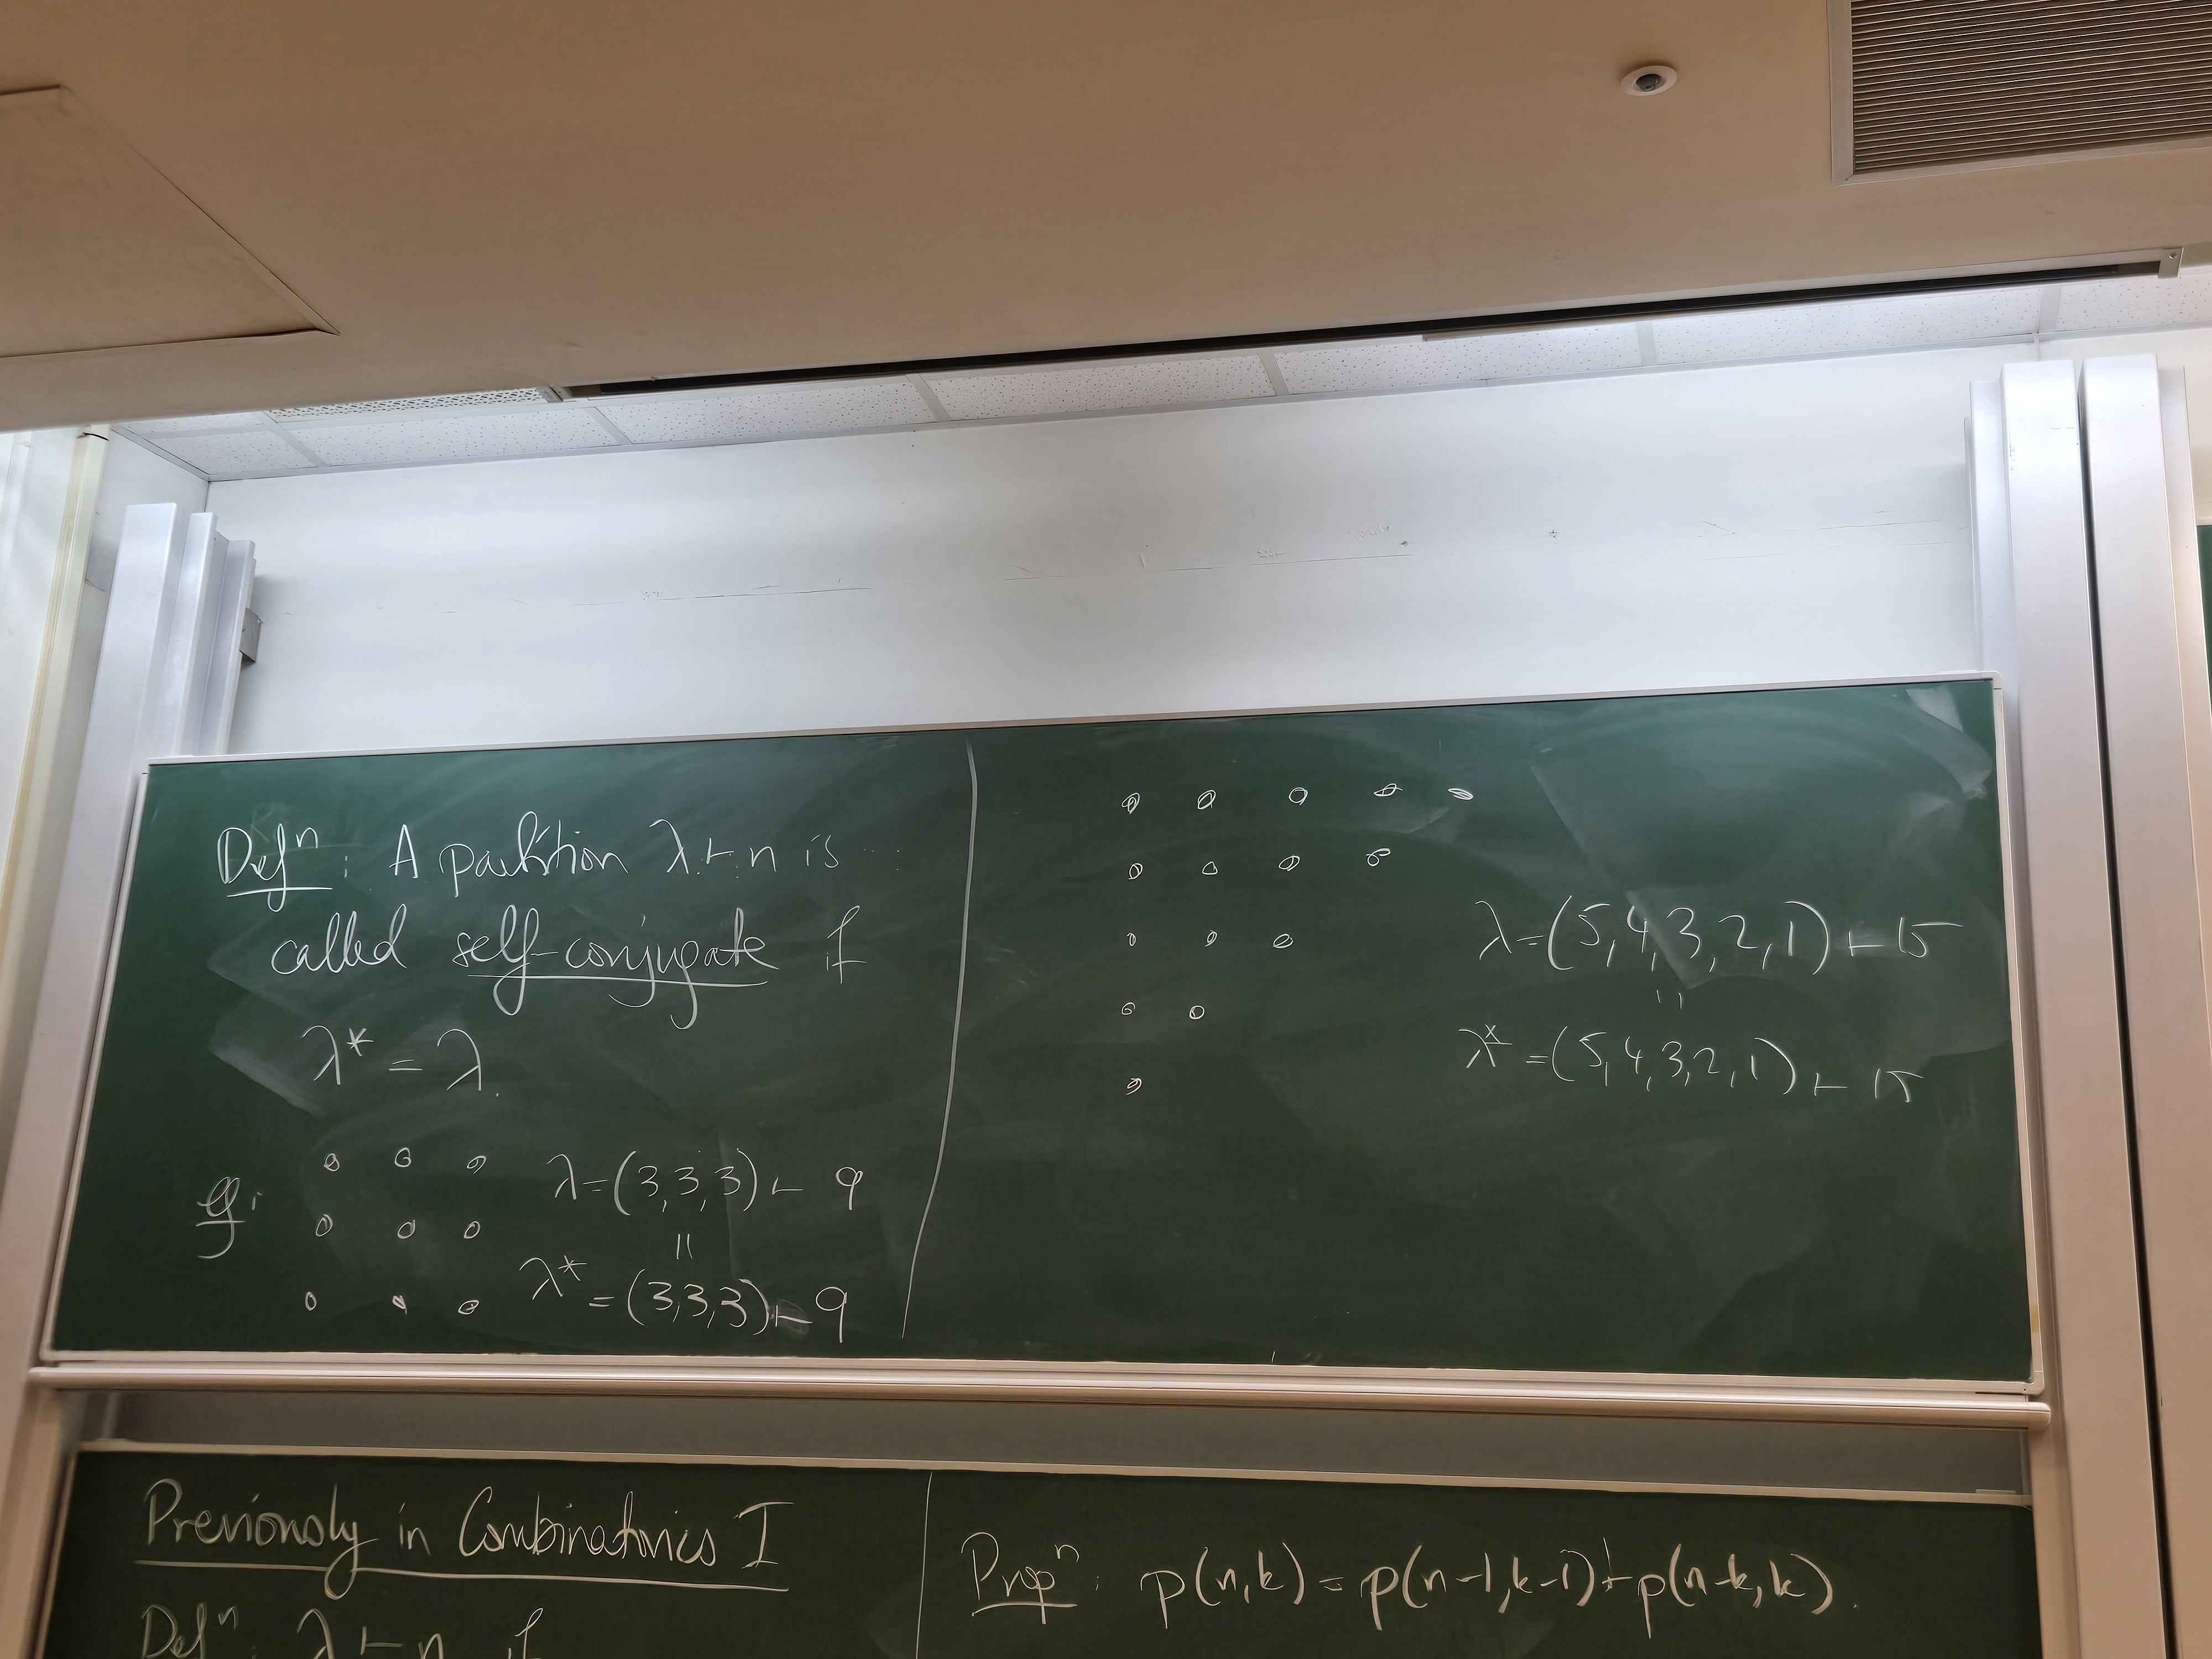
\includegraphics[width=0.8\textwidth]{./Figures/20250923_154927.jpg}
    \caption{Self-conjugate}
    \label{fig:self-conjugaet}
\end{figure}

\begin{proposition}
    The number of self-conjugate partition of \(n\) is the number of partition of \(n\) into distinct odd parts, which means
    \[
        (\lambda _1, \lambda _2, \dots , \lambda _k) : \lambda _1 > \lambda _2 > \dots > \lambda _k \ge 1, \quad \forall 1 \le i \le k, \ \lambda _i \equiv 1 \mod{2}.
    \]  
\end{proposition}
\begin{proof}
    Let \(\lambda \) be a self-conjugate partition. (See \autoref{fig: hook bijection}) If we consider the dots in the first row or column (we called it a hook), since \(\lambda = \lambda ^*\), we have \(2\lambda_1 - 1\) dots, which is an odd part. If we take the \(i\)-th part of the new partition to be the points in the \(i\)-th row or \(i\)-th column not-yer counted, then we get 
    \[
        (\lambda _i - (i - 1)) + (\lambda _i - (i - 1)) - 1,
    \]      say \(\mu _i = 2\left( \lambda _i - (i - 1) \right) - 1 \), then \(\mu \vdash n\) and
    \begin{align*}
        \mu _{i + 1} &= 2 \lambda _{i + 1} - 2(i + 1) + 1 \\
        &\le 2\lambda _i - 2(i + 1) + 1 \\
        &< 2\lambda _i - 2i + 1 = \mu _i,
    \end{align*}  
    so \(\mu \) has distinct parts and clearly \(\mu _i\) is odd for all \(i\). Hence, we have mapped our self-conjugate \(\lambda \) into a partition \(\mu \) with distinct odd parts. This is indeed a bijeciton.  
    \begin{figure}[H]
        \centering
        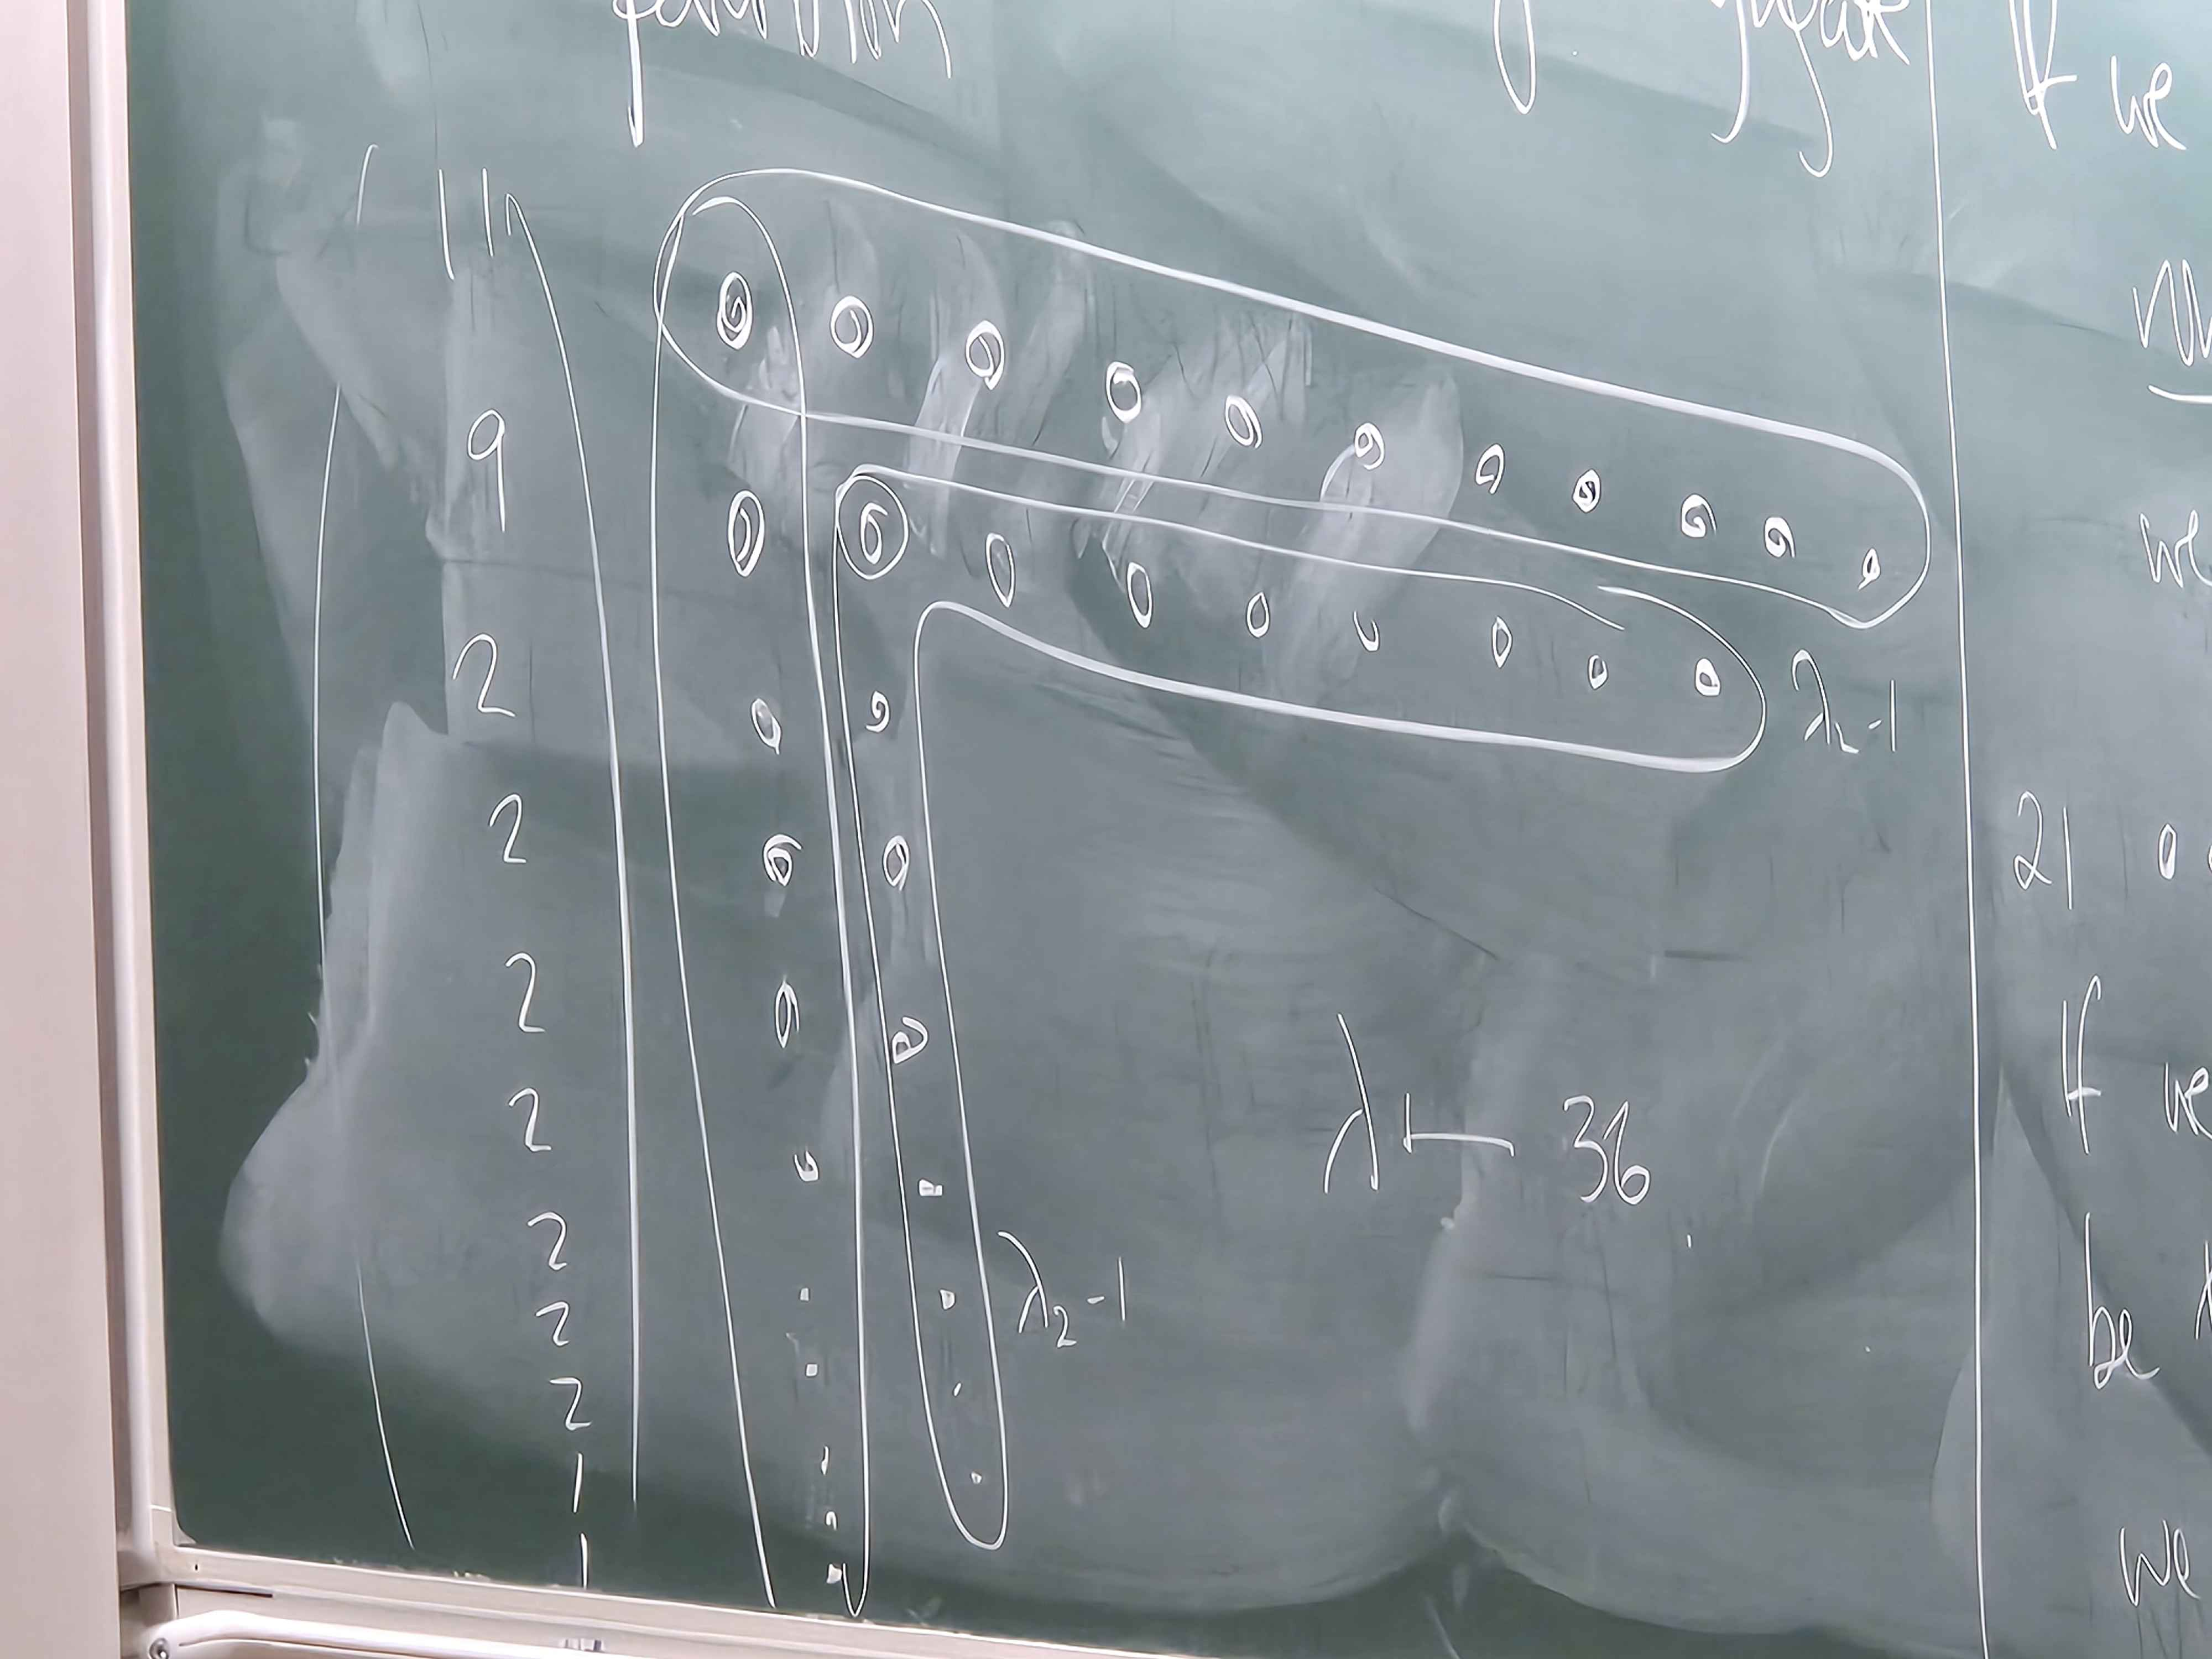
\includegraphics[width=0.8\textwidth]{./Figures/20250923_161129.jpg}
        \caption{Use hook to obtain bijection}
        \label{fig: hook bijection}
    \end{figure}
    
        
\end{proof}

\begin{figure}[H]
    \centering
    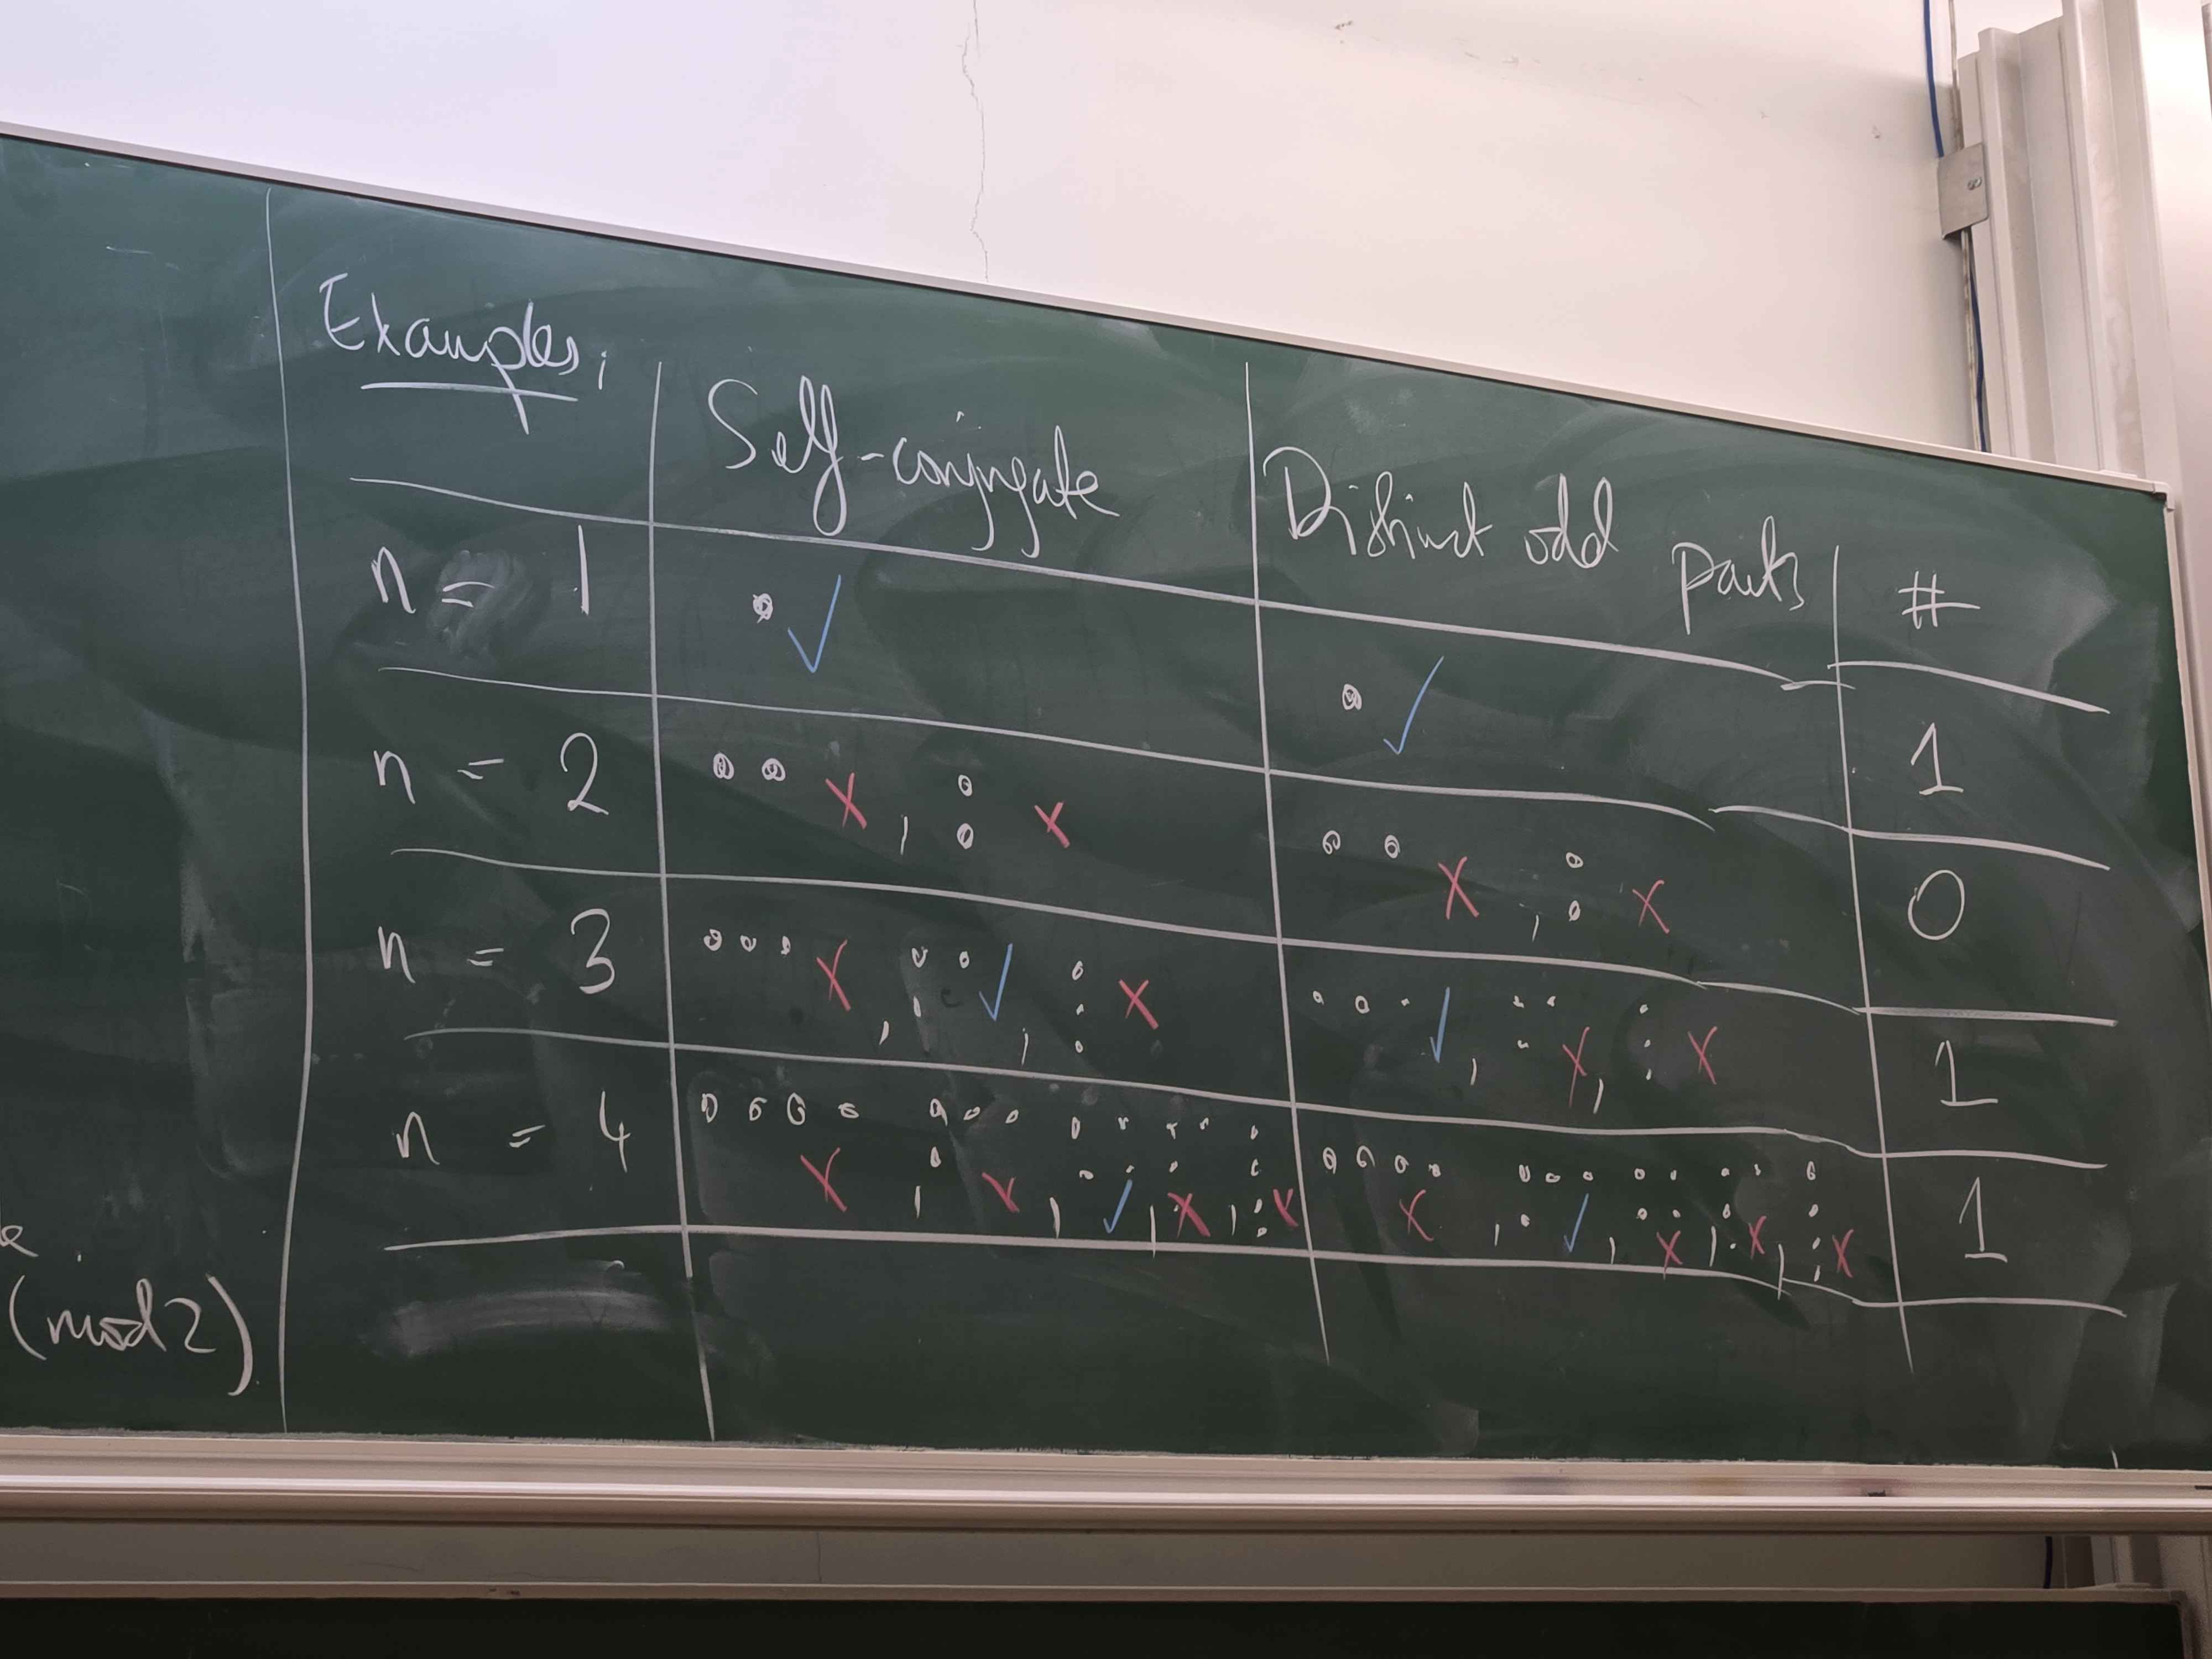
\includegraphics[width=0.8\textwidth]{./Figures/20250923_155744.jpg}
    \caption{Some cases of small \(n\).}
    \label{fig:self conjugate distinct odd part}
\end{figure}

\begin{eg}
    Square partition \(\lambda = \underbrace{(k, k, \dots ,k)}_{k \text{ parts}} \vdash k^2\) are self conjugate. 
\end{eg}

\begin{corollary}
    The sum of the first \(k\) odd numbers is \(k^2\).  
\end{corollary}
\begin{explanation}
    By drawing hooks, it is trivial.
    \begin{figure}[H]
        \centering
        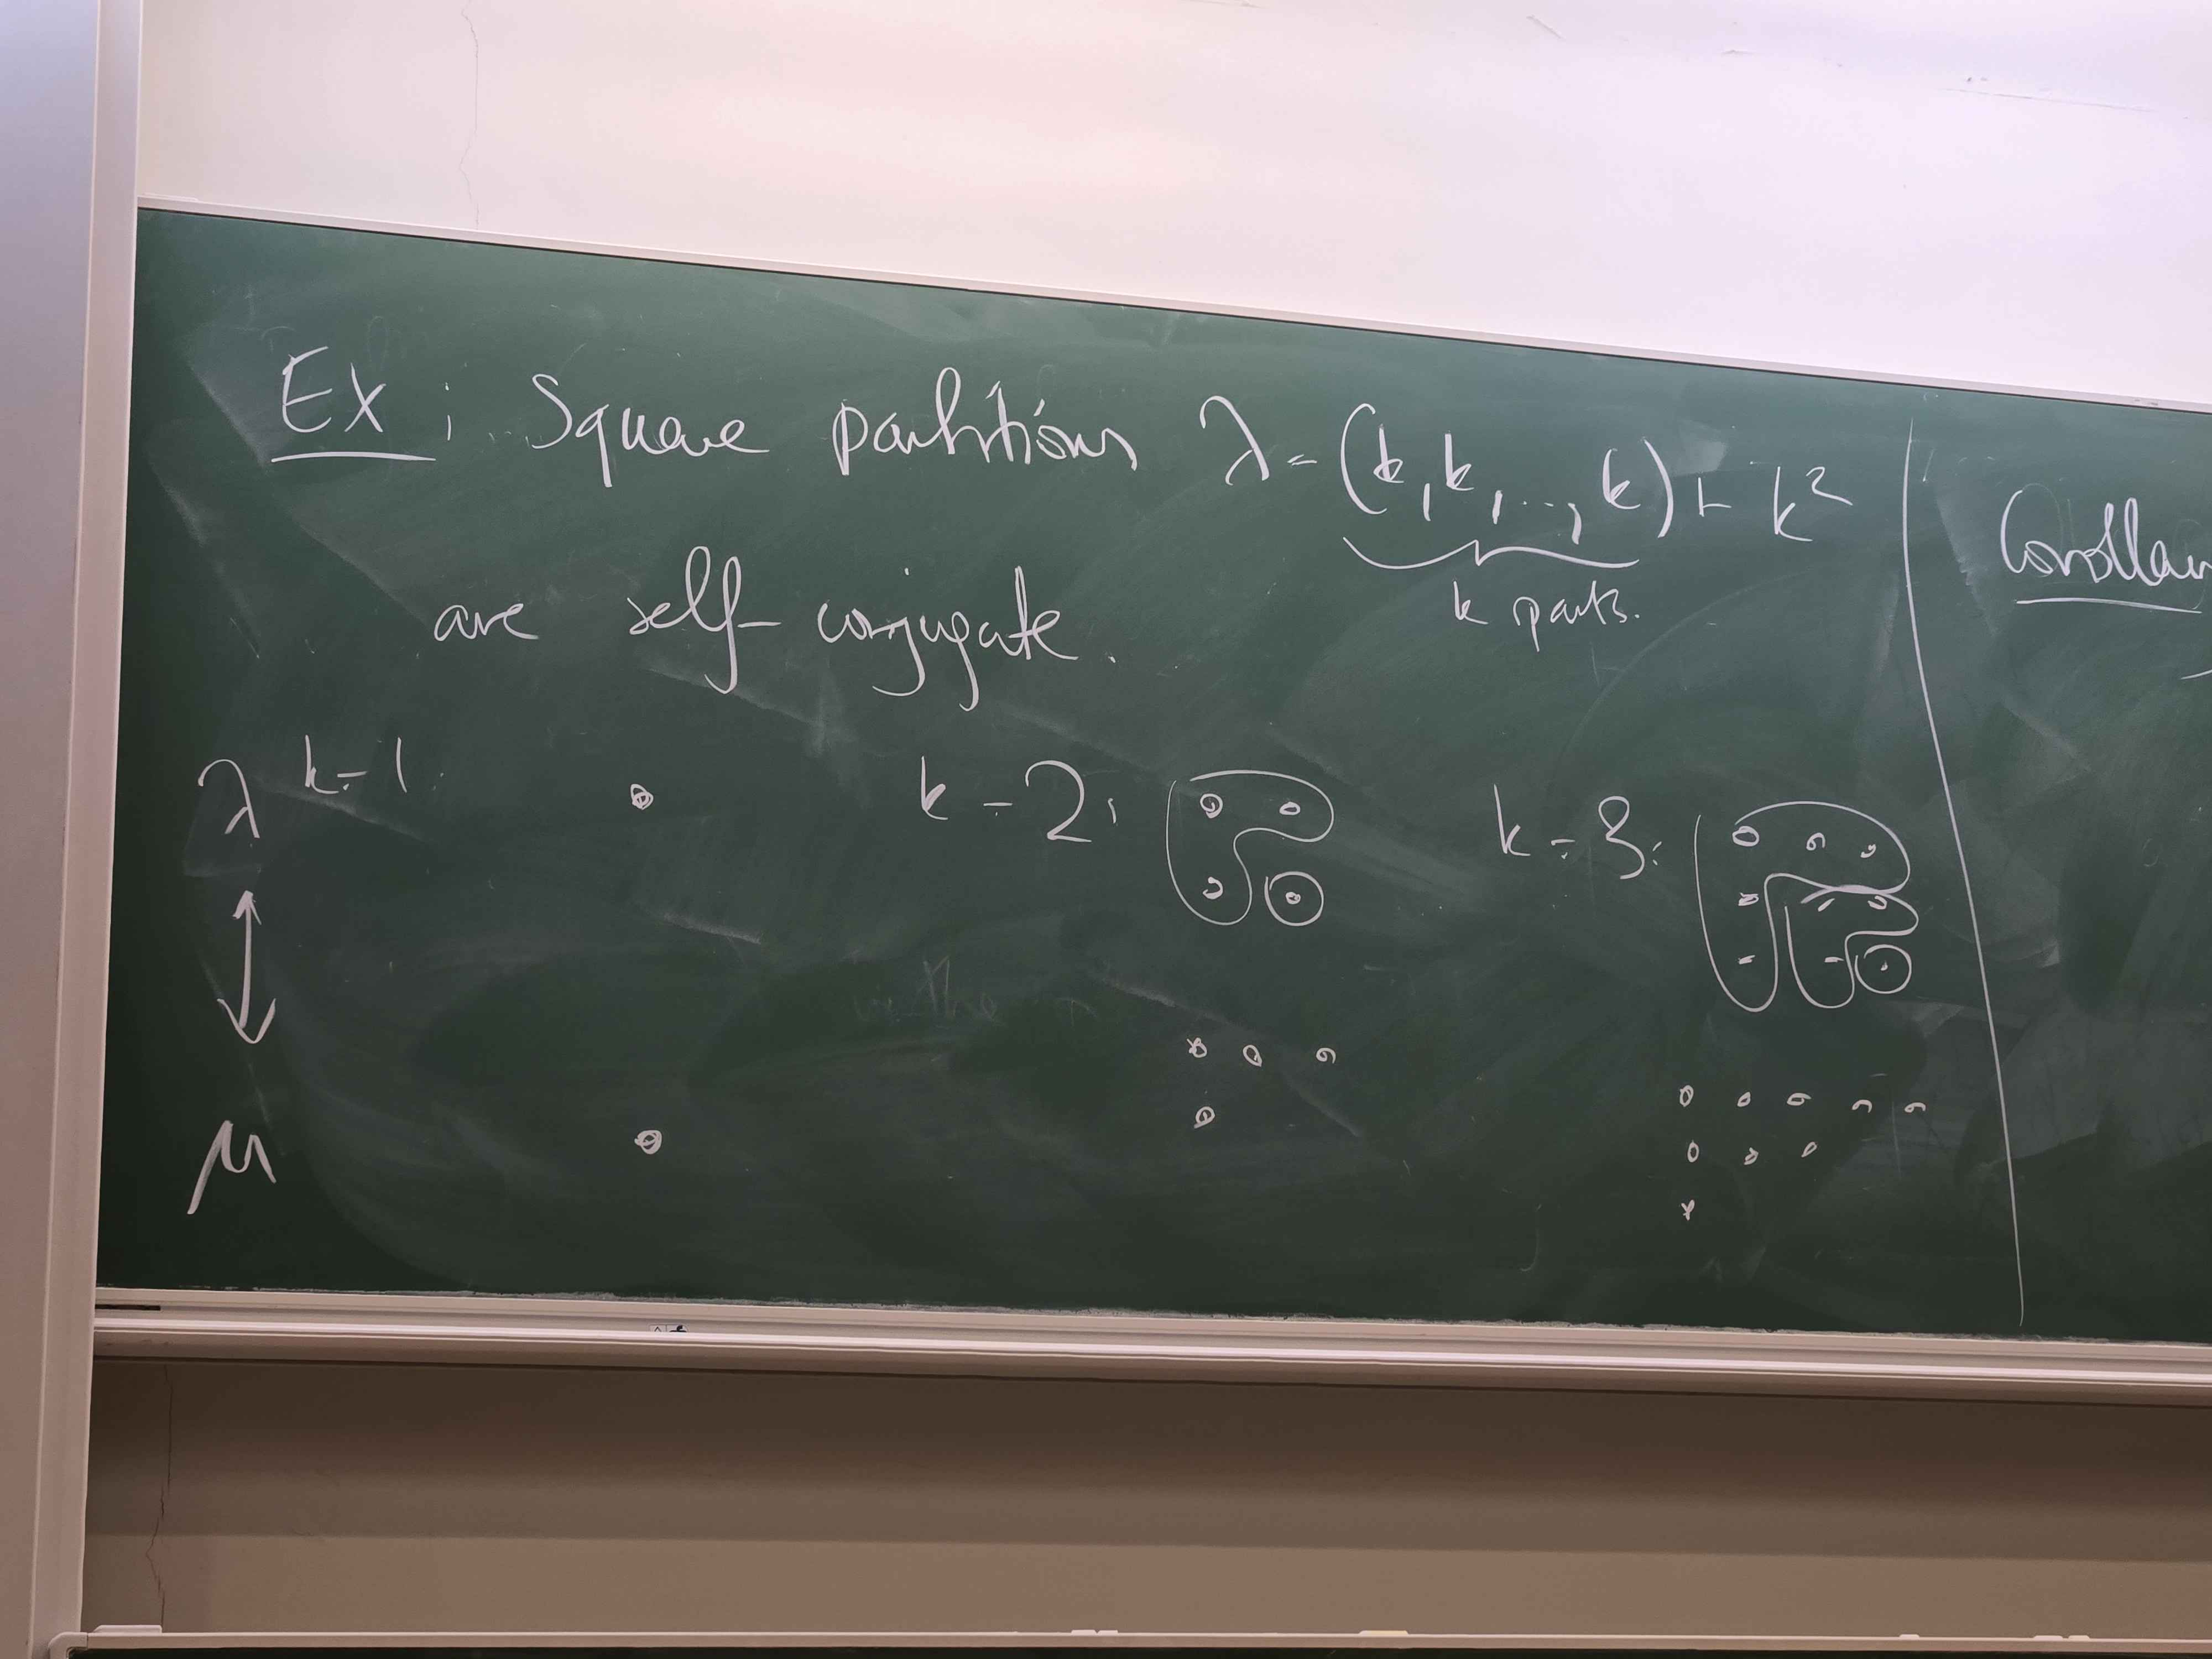
\includegraphics[width=0.8\textwidth]{Figures/20250923_161638.jpg}
        \caption{Drawing hooks to get the first \(k\) odd numbers from a square}
        \label{fig:first k odd sum is kk}
    \end{figure}
\end{explanation}
\section{The twelvefold way of Counting}
\begin{question}
    How many ways can we partition \(n\) items into \(k\) groups?  
\end{question}
\begin{table}[H]
    \centering
    \begin{tabular}{c|c|c}
        \toprule
            Itmes & Groups & Partition  \\
        \midrule
            numbered &  numbered& injective(group of size \(\le 1\))  \\
            indistinguisable &  indistinguishable&  surjective(group of size \(\ge 1\))  \\
            && arbitrary \\
        \bottomrule
    \end{tabular}
    \caption{All types of partition problem.}
    \label{tab:type of partition problem}
\end{table}

\begin{table}[H]
    \centering
    \begin{tabular}{c|c|c|c}
        \toprule
             & Injective & Surjective & Arbitrary   \\
        \midrule
            Items, groups numbered & \(k^{\underline{n}}\)  & \(S(n, k) \cdot k!\)  & \(k^n\)   \\
            \midrule
            Items numbered, groups not & \(\begin{dcases}
                1, &\text{ if }  k \ge n;\\
                0, &\text{ if }  k < n.
            \end{dcases}\)  & \(S(n, k)\)  & \(\sum_{j=0}^k S(n, j) \)   \\
            \midrule
            Items not, groups numbered & \(\binom{k}{n}\)  & \(\binom{n - 1}{k - 1}\)  &  \(\binom{n + k - 1}{k - 1}\)  \\
            \midrule
            Items, groups not numbered &\(\begin{dcases}
                1, &\text{ if }  k \ge n;\\
                0, &\text{ if }  k < n.
            \end{dcases}\) & \(p(n, k)\) & \(\sum_{j=0}^k p(n, j) \) \\
        \bottomrule
    \end{tabular}
    \caption{All solution to all kinds of partition problem}
    \label{tab:all sol to partition problem}
\end{table}

\chapter{Generating Functions}
\begin{figure}[H]
    \centering
    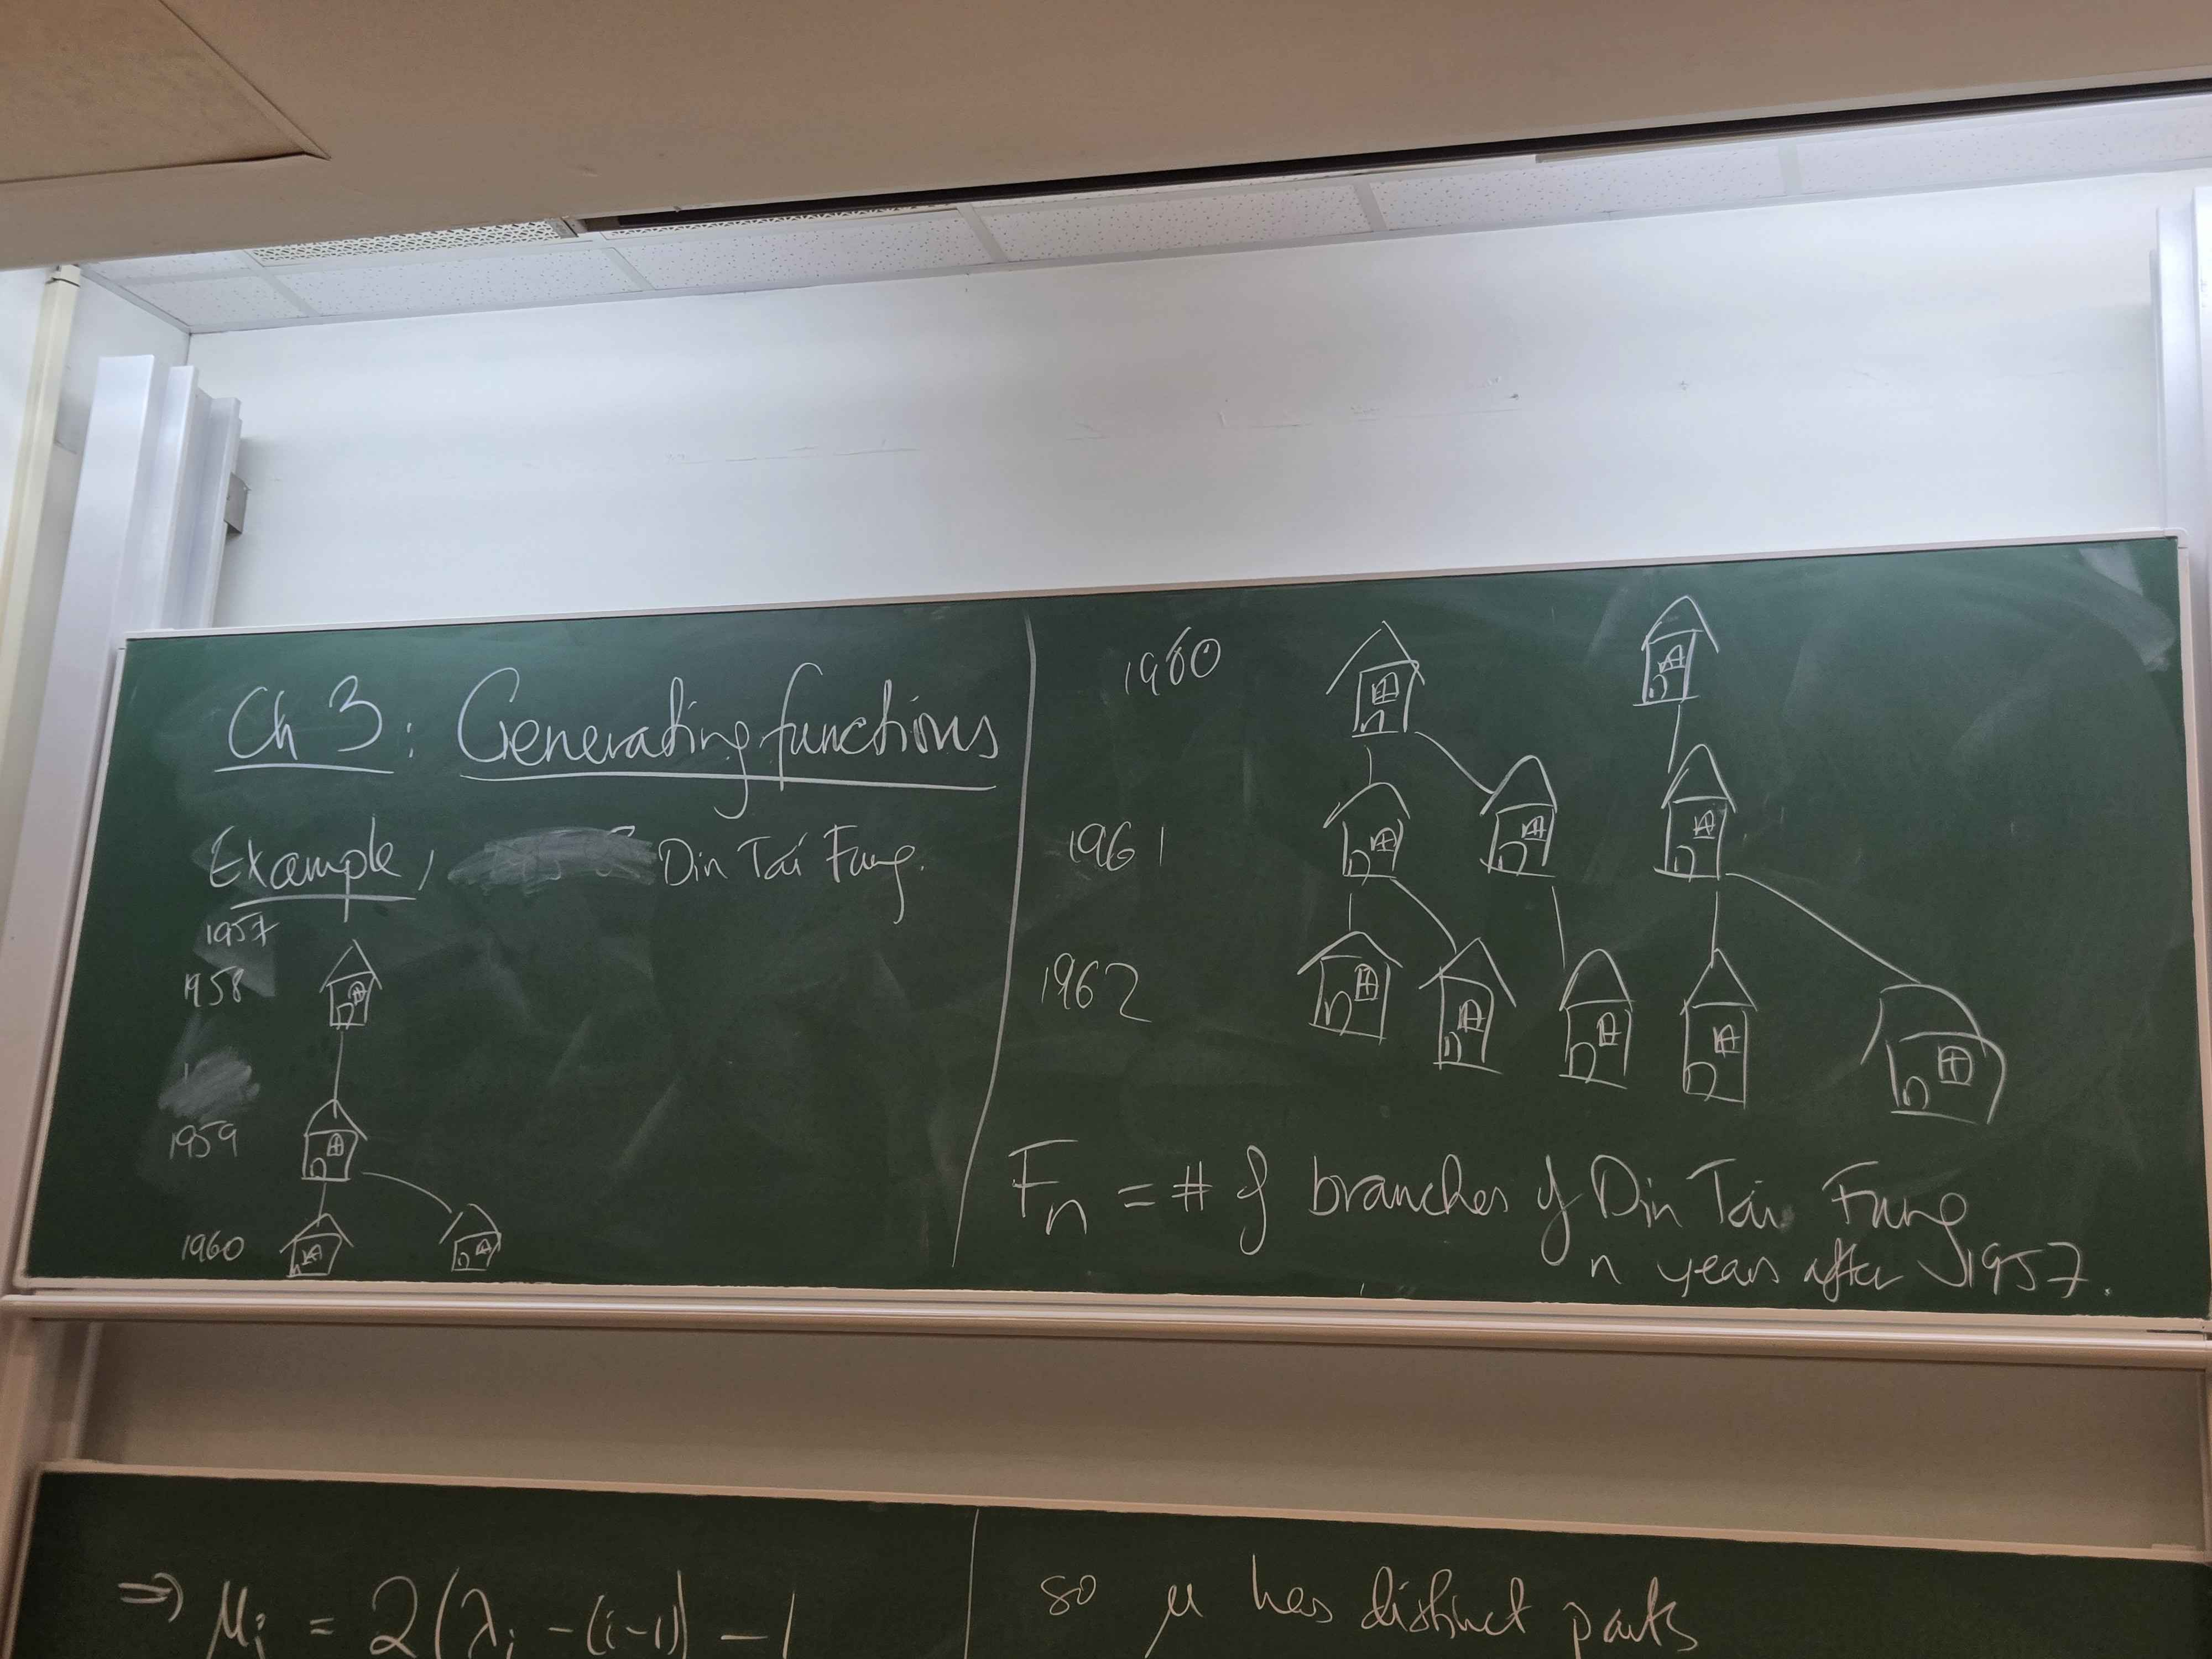
\includegraphics[width=0.8\textwidth]{./Figures/20250923_165742.jpg}
    \caption{Din Tai Fung branches number}
    \label{fig: fibonacci from ding tai fung}
\end{figure}

We have a recurrence relation: \(\forall n \ge 2\)
\[
    F_n = F_{n - 1}+ F_{n -2}
\] 

\begin{eg}
    If 
    \[
        F_n ^{\prime}  = F_{n-1}^{\prime} + F_{n-1}^{\prime}, 
    \] then \(F_n^{\prime} = 2^n F_0^{\prime} \). 
\end{eg}

Suppose \(\left\{ F_n \right\}_{n=1}^{\infty}  \) is a recurring sequence, then we can define a power series as 
\[
    F(x) = F_0 + F_1 x + F_2 x^2 + \dots = \sum_{n=0}^{\infty} F_n x^n. 
\] 

Thus, we have 
\[
    xF(x) = F_0 x + F_1 x^2 + \dots = \sum_{n=0}^{\infty} F_n x^{n + 1} = \sum_{n=1}^{\infty} F_{n-1} x^n.  
\]
If we do it again, then we can get 
\[
    x^2 F(x) = F_0 x^2 + F_1 x^3 + \dots = \sum_{n=0}^{\infty} F_n x^{n + 2} = \sum_{n=2}^{\infty} F_{n - 2} x^n.  
\]
Now we have 
\[
    F(x) - xF(x) - x^2 F(x) = F_0 x^0 - F_1 x^1 - F_0 x^1 + \sum_{n = 2}^{\infty} \underbrace{\left( F_n - F_{n - 1} - F_{n-2} \right)}_{=0} x^n = 0. 
\]
Hence, \((1 - x - x^2) F(x) = x\), and thus 
\[
    F(x) = \frac{x}{1 - x - x^2} = \frac{A}{1 - \alpha _1 x} + \frac{B}{1 - \alpha _2 x}.
\] 
Now we solve the \(A, B, \alpha _1, \alpha _2\). 
\begin{align*}
    \frac{A}{1 - \alpha _1} + \frac{B}{1 - \alpha _2} &= \frac{A(1 - \alpha _2 x) + B(1 - \alpha _1 x)}{(1 - \alpha _1 x)(1 - \alpha _2 x)} \\
    &= \frac{(A + B) - (A \alpha _2 + B \alpha _1)x}{1 - (\alpha _1 + \alpha _2)x + \alpha _1 \alpha _2 x^2} = \frac{x}{1 - x - x^2}.
\end{align*} 

Hence, we want 
\[
    \begin{dcases}
        A + B = 0 \\
        A \alpha _2 + B \alpha _1 = -1 \\
        \alpha _1 + \alpha _2 = 1 \\
        \alpha _1 \alpha _2 = -1 \\
    \end{dcases},
\]
 by solving \(\alpha _1, \alpha _2\) first, we can get \(\alpha _1 = \frac{1 + \sqrt{5} }{2}\) and \(\alpha _2 = \frac{1 - \sqrt{5} }{2}\), and thus we can solve \(A = \frac{1}{\sqrt{5} }\) and \(B = -\frac{1}{\sqrt{5} }\). Hence, we have 
 \[
    F(x) = \frac{x}{1 - x - x^2} = \frac{\frac{1}{\sqrt{5} }}{1 - \left( \frac{1 + \sqrt{5} }{2} \right)x } - \frac{\frac{1}{\sqrt{5} }}{1 - \left( \frac{1 - \sqrt{5} }{2} \right)x }. 
 \]

 Now since we know 
 \[
    \frac{1}{1- \alpha } = 1 + \alpha + \alpha ^2 + \dots ,
 \]so we can get 
\begin{align*}
    F(x) &= \frac{1}{\sqrt{5} } \left( \left( 1 + \left( \frac{1+\sqrt{5} }{2} \right)x + \left( \left( \frac{1+\sqrt{5} }{2} \right)x \right)^2  + \dots   \right) - \left( 1 + \left( \frac{1 - \sqrt{5} }{2}x + \left( \left( \frac{1-\sqrt{5} }{2} \right)x \right)^2+ \dots  \right)  \right)   \right) \\ &= \frac{1}{\sqrt{5} } \sum_{n=0}^{\infty} \left( \left( \frac{1 + \sqrt{5} }{2} \right)^n - \left( \frac{1 - \sqrt{5} }{2} \right)^n  \right) x^n = \sum_{n=0}^{\infty} F_n x^n.   
\end{align*}

Hence, we have 
\[
    F_n = \frac{1}{\sqrt{5} } \left( \left( \frac{1 + \sqrt{5} }{2} \right)^n - \left( \frac{1 - \sqrt{5} }{2} \right)^n   \right). 
\]